\documentclass[tikz,border=10pt]{standalone}
\usepackage{tikz}
\usepackage{amsmath}

\begin{document}

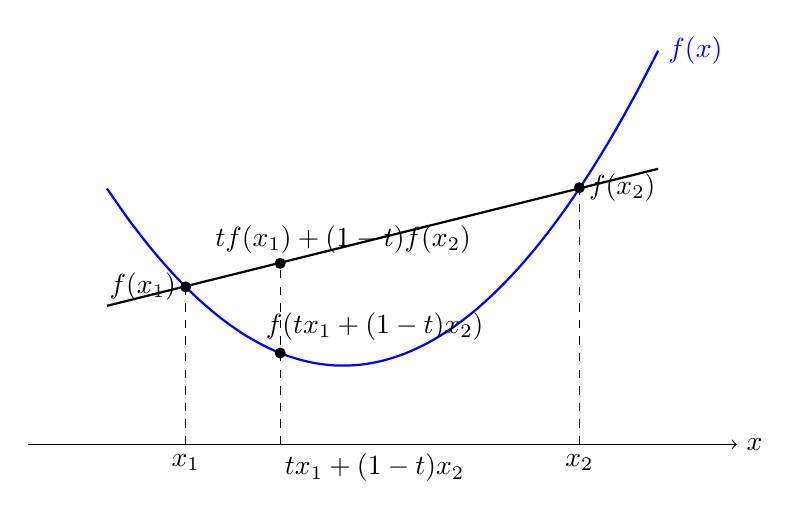
\begin{tikzpicture}[scale=2]
    \draw[->] (0, 0) -- (4.5, 0) node[right] {$x$};
    
    \draw[thick, domain=0.5:4, smooth, variable=\x, blue] plot ({\x}, {0.5*(\x-2)*(\x-2) + 0.5}) node[right] {$f(x)$};
    
    \fill (1,1) circle (1pt) node[left] {$f(x_1)$};
    \draw[dashed] (1,0) node[below] {$x_1$} -- (1,1);

    \fill (3.5,1.63) circle (1pt) node[right] {$f(x_2)$};
    \draw[dashed] (3.5,0) node[below] {$x_2$} -- (3.5,1.6);

    \fill (1.6,0.58) circle (1pt);
    \fill (1.6,1.15) circle (1pt);
    \draw[dashed] (1.6, 0) -- (1.6,1.15);
    \node[below] at (2.2, 0) {$t x_1 + (1-t) x_2$};
    \node[above] at (2.2,0.6) {$f(t x_1 + (1-t)x_2)$};
    \node[above] at (2.0,1.15) {$tf(x_1) + (1-t)f(x_2)$};

    \draw[thick] (0.5, 0.88) -- (4, 1.75);
\end{tikzpicture}

\end{document}